\newpage
\subsubsection{Caso d'uso UC4.3: Login Tramite Twitter }
\label{UC4_3}
\begin{figure}[ht]
	\centering
	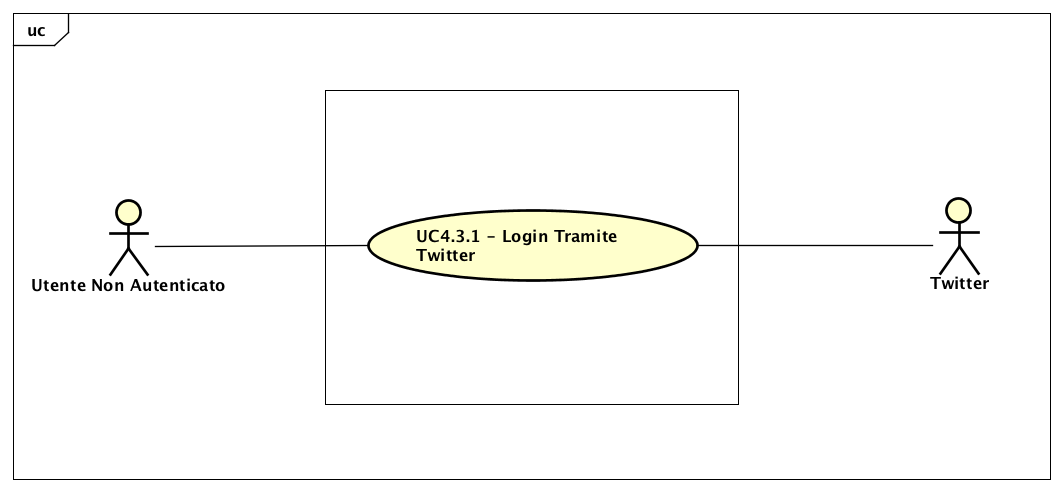
\includegraphics[scale=0.45]{UML/UC4_3.png}
	\caption{UC4.3: Login Tramite Twitter}
\end{figure}

\begin{longtable}{ l | p{11cm}}
	\hline
	\rowcolor{Gray}
	 \multicolumn{2}{c}{UC4.3 - Login Tramite Twitter} \\
	 \hline
	\textbf{Attori} & Utente Non Autenticato, Twitter \\
	\textbf{Descrizione} & L'utente non autenticato effettua il login all'applicazione web tramite Twitter, così da evolversi in un utente autenticato\\
	\textbf{Pre-Condizioni} & L'utente ha scelto di eseguire il login all'applicazione web e non è autenticato \\
	\textbf{Post-Condizioni} & L'utente ha effettuato il login all'applicazione web tramite Twitter, evolvendosi in un utente autenticato \\
	\textbf{Scenario Principale} & \begin{enumerate*}[label=(\arabic*.),itemjoin={\newline}]
		\item L'utente non autenticato può effettuare il login all'applicazione web tramite Twitter (UC4.3.1)
	\end{enumerate*}\\
\end{longtable}